\section{Projektdaten und -ziele}\label{sec:projektdaten}

Das Ziel der Projektarbeit ist es, einen stabil laufenden Prototyp des Twin-Stick Shooters\footnote{
Zur Genreeinteilung siehe auch \cite[]{GameDeveloper}
} \textit{Geometry Wars} (siehe Abbildung~\ref{fig:geometry_wars}) unter Verwendung der Programmiersprache \textit{C++} (23) und der OpenGL-API~\cite[]{OpenGLHomepage} zu erstellen.

\begin{figure}[tbp]
    \centering
    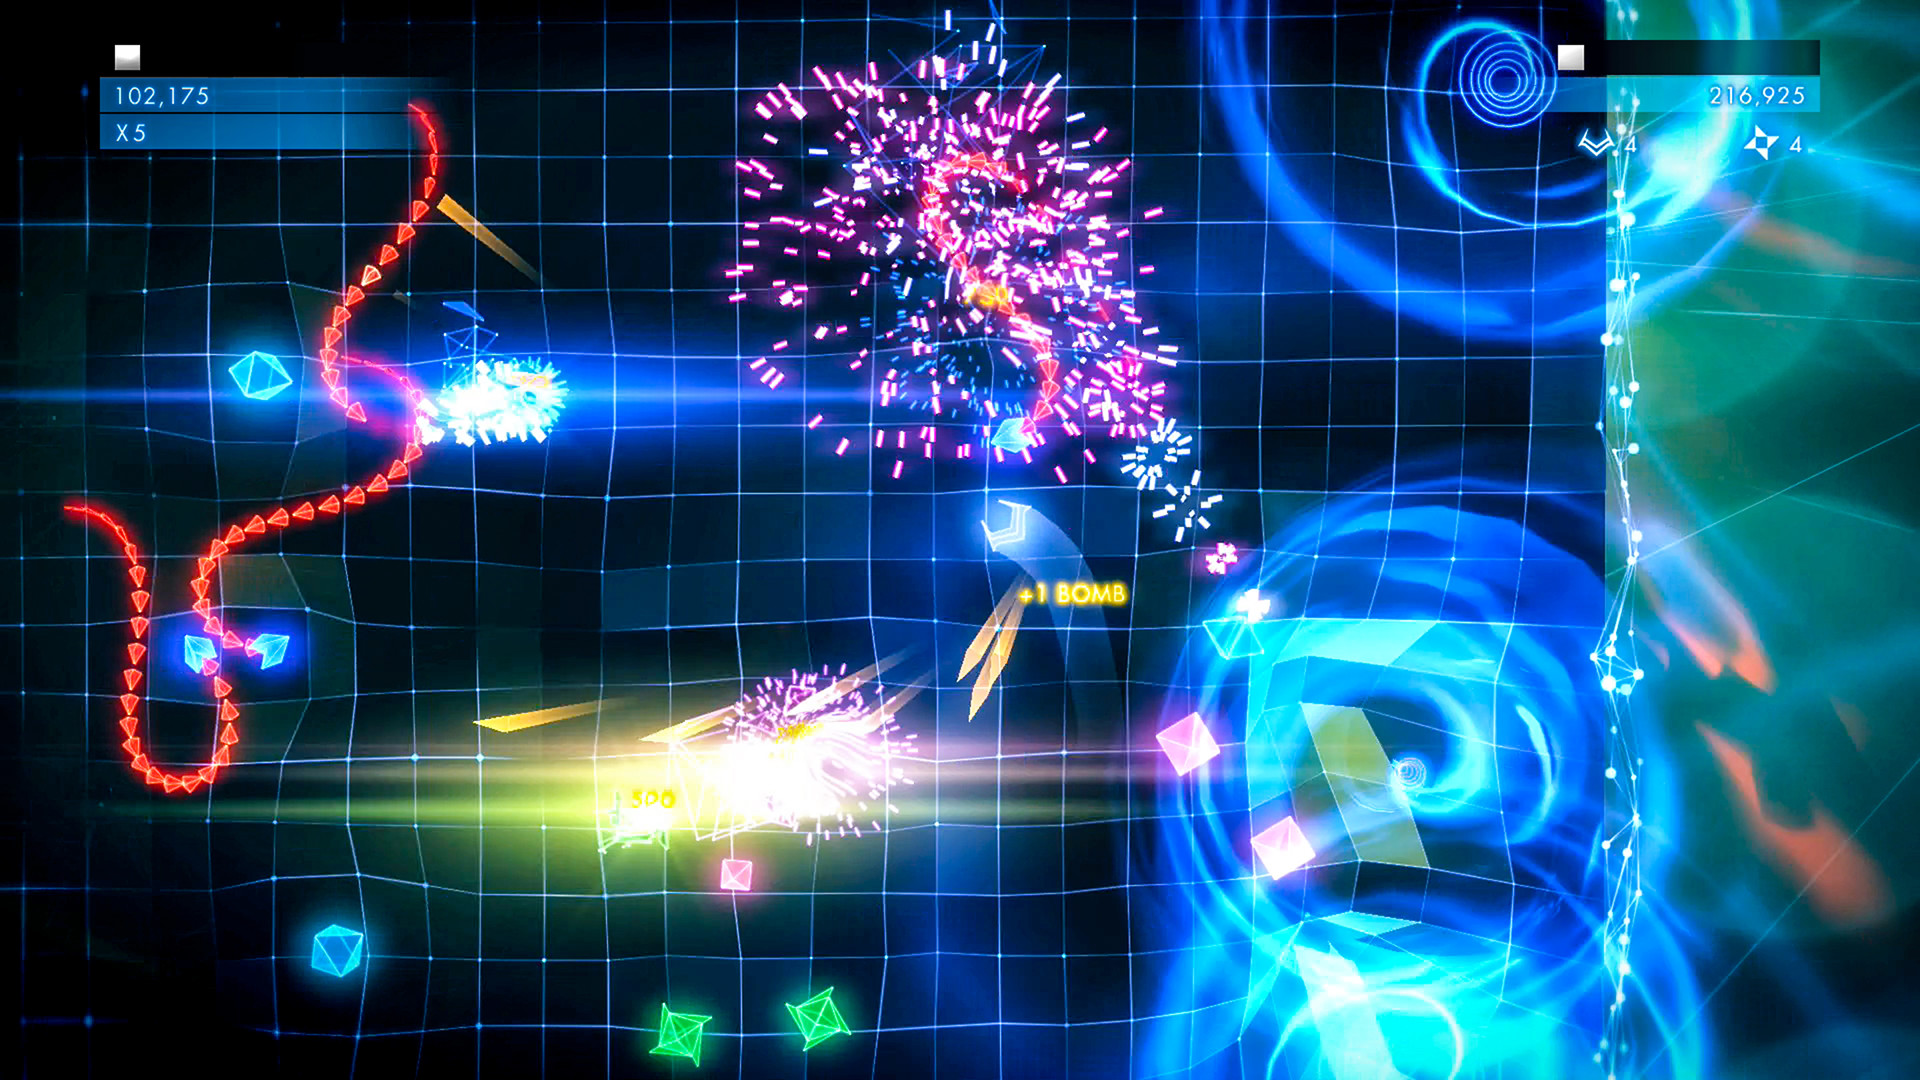
\includegraphics[width=1\columnwidth]{img/geometry_wars}
    \caption{Geometry Wars fand sich erstmals 2003 als Easter Egg in dem Spiel \textit{Project Gotham Racing} (Microsoft Game Studios). Aufgrund der großen Beliebtheit entstanden mehrere Nachfolger, zuletzt 2016 mit \textit{Geometry Wars 3: Dimensions Evolved} (Activision). (Quelle: Steam)}
    \label{fig:geometry_wars}
\end{figure}



Als zu realisierende Features wurden vereinbart (siehe Anhang~\ref{sec:projektvorschlag}):


\begin{itemize}
    \itemsep0.5em
    \item Spielbares Level (2D-Grid)
    \item Time-Attack Modus mit einer Dauer von 3 Minuten
    \item Highscore-System
    \item Controller-Steuerung
    \item Stabile Framerate von mindestens 60 FPS bei gleichzeitiger Darstellung von über hundert Gegnern und Objekten
    \item Drei Gegnertypen mit einfacher KI (``Spawn and Chase``)
    \item Aufwertung des Game Feels durch grafische Effekte
    \item Compilierbar und lauffähig unter Windows 11
\end{itemize}


Während einige Kriterien konkret messbar sind (Framerate), sind andere Anforderungen bewusst unscharf formuliert (Game Feel) und unterstreichen den explorativen Charakter des Projekts.
Ein Requirements Engineering ist folglich nicht Bestandteil der Arbeit, zumal auch das Original-Spiel, an dem sich die Umsetzung orientiert, als ein Maßstab dienen soll.\par

Der Lernprozess wird im Besonderen als ein wesentliches Ziel dieser Arbeit betrachtet, für dessen Bewertung keine formalen Metriken herangezogen werden.
Stattdessen sollen die gewonnenen Erfahrungen und Ergebnisse im Anschluss schriftlich festgehalten und das hier vorliegende Dokument kritisch reflektiert werden.\par

Vor diesem Hintergrund wird das Vorgehen als eine Form des dynamischen Requirements Engineering ``mit deutlich größeren Freiheitsgeraden``~\cite[60]{MRP21} betrachtet: Das erwähnte \textit{Tracer Bullet Development}, das vor allem eine Plattform zur Integration bereitstellt, entspricht dem von \textit{Pflug et al.} mit ``Living Lab`` bezeichneten Prototyp, der im Weiteren nach agilen Methoden entwickelt wird (\textit{ebd., S. 61})\footnote{
    Kasurinen et al. gehen in~\cite[]{KMS14} der Frage nach, ob das im Ingenieursbereich angesiedelte Anforderungsmanagement bei der stark durch kreative Prozesse beeinflussten Spieleentwicklung einen Platz hat. Sie zeigen, dass befragte Entwickler einen Teil der Anforderungen an ihr Spiel ganz bewusst erst durch \textit{User Testing} ableiten. Entsprechend stellt \textit{Games User Research} einen wichtigen Zweig der Spieleindustrie dar, der Unternehmen dabei unterstützt, Spiele-Erfahrung zu verstehen und zu verbessern (vgl.~\cite[26]{Zam18}). Weitere Diskussionen bzgl. Herausforderungen beim Software Engineering bei der Spielentwicklung in~\cite[]{KH09}.
}, und ein Einbringen eigener kreativer Ideen erlauben soll.\\

\subsection{Zeitplan}

Wir stellen den Zeitplan und die zugehörigen Meilensteine in Tabelle~\ref{tab:zeitplan} vor.
Die dort angegebene zeitliche Gliederung dient der Orientierung zur Umsetzung; die sequentielle Auflistung impliziert kein Wasserfallmodell.

\setlength{\tabcolsep}{8pt}
\begin{table}[t]
    \centering
    {\renewcommand{\arraystretch}{1.2}%
    \begin{tabularx}{\textwidth}{@{} l l Y @{}}
        \toprule
        \textbf{Meilenstein} & \textbf{Datum} & \textbf{Inhalt} \\
        \midrule
        \texttt{milestone\_1} & 20.10.2025 &
        Bereitstellung der Applikationsschicht inkl. Implementierung des Event-Systems,
        des Input-Managers sowie Anbindung an das Low-Level-API-Subsystem. \\
        \texttt{milestone\_2} & 17.11.2025 &
        Bereitstellung der Rendering-Engine; erster Entwurf des Spielfelds samt Darstellung des Spielerschiffs. \\
        \texttt{milestone\_3} & 22.12.2025 &
        Umsetzung der Physik und Spielereingabe zur Steuerung des Schiffs; Feuermechaniken. \\
        \texttt{milestone\_4} & 19.01.2026 &
        Implementierung der wichtigsten Spielregeln und -mechaniken; spielfähiger Prototyp. \\
        \texttt{milestone\_5} & 09.02.2026 &
        Bereitstellung des Prototyps; Feinschliff. \\
        \texttt{milestone\_6} & 16.03.2026 &
        Abgabe der Dokumentation und Vorstellung des Projekts. \\
        \bottomrule
    \end{tabularx}}
    \caption{Geplante Meilensteine zur Umsetzung des Geometry Wars Klon.
    Zum Zeitpunkt der Veröffentlichung dieses Dokumentes ist der erste Meilenstein abgeschlossen: helios bietet bereits ein einfaches Fenstermanagement, rudimentäre Eingabe-Verarbeitung, ein Logging-System sowie ein funktionierendes Rendering Layer samt Anbindung an die OpenGL-API.}
    \label{tab:zeitplan}
\end{table}



\noindent
Mit der Vorgabe des umzusetzenden Spielkonzeptes entfällt ein damit verbundenes Prototyping.
Die gegenwärtige Entwicklungsphase ordnen wir als die \textit{hard-architecture design}-Phase ein und folgen damit Rollings und Morris~\cite[628]{RM04}.\par

Das Projekt ist unter der MIT-Lizenz  auf Github veröffentlicht, Source Code und Ticketsystem sind öffentlich einsehbar~\cite[]{heliosgithub}.\par


